
\begin{eqnarray*}
    I_{m} &=& \frac{E_{m}}{\sqrt{R^{2} + (L \omega -\frac{1}{c \omega })^{2}}} \\
    \implies U_{m} &=& R \cdot I_{m} = \frac{E}{D}  \\ 
    \text{ avec } D &=& \sqrt{1+Q^{2}(x-\frac{1}{x})^{2}} \text{ avec } x = \frac{\omega }{\omega _{0}} \text{ et } Q = \frac{L \omega_{0}}{R}
\end{eqnarray*}


Il y a donc une résonance en intensité pour toute valeur de \(Q\) et la pulsation de résonance est indépendante de \(Q\) 
\begin{definition}[Bande passante]
    Soient \(\omega_{1}\) et \(\omega _{2}\) définis par : 
    \[
        I_{m}(\omega = \omega _{1}) = I_{m}(\omega = \omega_{2}) = \frac{I_{\max }}{\sqrt{2}}
    \]  
    et : 
    \[
        I_{m, \max } = I_{m} (\omega = \omega _{0}) = \frac{E}{R}
    \]
\end{definition}

\begin{remark}[rem]
    \[
        I_{m} = \frac{E}{\sqrt{R^{2} + (L \omega - \frac{1}{c \omega })^{2}}}
    \]
\end{remark}
\begin{corollary}[Valeurs de \(\omega_{1}\) et \(\omega_{2}\) ]
    On cherche à calculer \(\omega_{1}\) et \(\omega_{2}\)  
    \begin{eqnarray*}
        I_{m}(\omega ) &=& \frac{E_{m}}{\sqrt{L}R} \\
        \implies R \sqrt{2} &=& \sqrt{R^{2} + (L \omega -\frac{1}{c \omega })^{2}} \\
        \implies 2R^{2} &=& R^{2} + (L \omega -\frac{1}{c \omega })^{2} \\
        \implies R^{2} &=& (L \omega -\frac{1}{c \omega })^{2} \\
        \implies  (L \omega -\frac{1}{c \omega })  &=& \pm R \\
        \implies  Lc \omega^{2} \pm RC \omega  -1 &=& 0 \\
        \implies \omega^{2} \pm \frac{R}{L} \omega - \omega_{0}^{2} &=& 0
    \end{eqnarray*}
    \begin{eqnarray*}
        \implies &&\text{ 2 solutions : } \\
        \implies \omega  &=& \frac{-\frac{R}{L} \pm \sqrt{(\frac{R}{L})^{2} + 4\omega^{2}}}{2} \\
        \text{ or } \omega &=& 2 \pi f \geq 0 \\
        \implies w_{1} &=& -\frac{R}{2L} + \frac{1}{2} \sqrt{\frac{R}{L}^{2} + 4 \omega_{0}^{2}} \\
        \text{ De même : } && \\
        \omega^{2} -\frac{R}{L} \omega - \omega_{0}^{2} &=& 0 \\
        \implies \omega &=& \frac{\frac{R}{L} \pm \sqrt{\frac{R}{L}^{2} + 4\omega _{0}^{2}}}{2} = 0 \\
        \implies  \omega _{2} &=& \frac{R}{2L} +\frac{1}{2}\sqrt{\frac{R}{L}^{2} + 4\omega_{0}^{2}}
    \end{eqnarray*}
\end{corollary}


\begin{definition}[Largeur de la bande passante] On définiy la lageur de la bande passante comme suit : 
    \[
        \Delta \omega = \omega_{2} - \omega _{1} = \frac{R}{L}
    \]
    On peut en déduire une version adimensionnée : 
    \[
        \frac{\Delta \omega }{\omega_{0}} = \frac{R}{L} \times \sqrt{LC} = \frac{R\sqrt{C}}{\sqrt{L}}
    \]
    Or : \(Q = \frac{L \omega _{0}}{R} = \frac{L}{R} \times \frac{1}{\sqrt{LC}} = \frac{\sqrt{L}}{R\sqrt{C}}\) 
    D'où : 
    \[
        \frac{\Delta \omega }{\omega _{0}} = \frac{1}{Q}
    \]
\end{definition}

\begin{figure}[!htb]
    \centering
    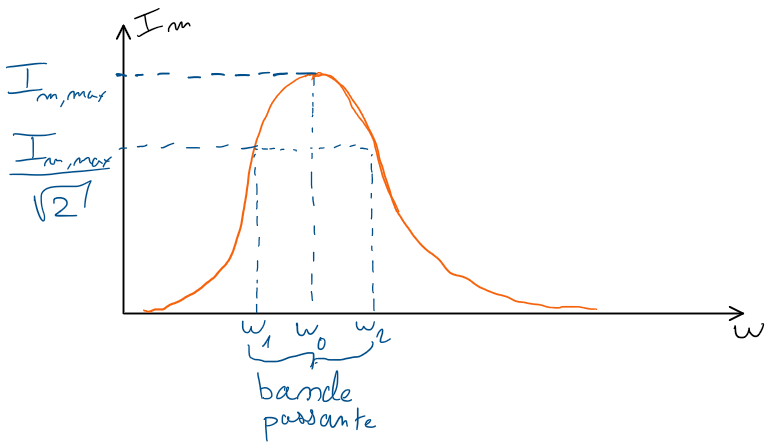
\includegraphics[width=1\textwidth]{SCHEMA12.png}
    \caption{Représentation de \(I_{m}\) en fonction de \(\omega\)}
    \label{fig:SCHEMA12}
\end{figure}

\begin{eqnarray*}
    \varphi = \arg \underline{I_{m}} \\
    \underline{I_{m}} = \frac{E}{R + j(L \omega -\frac{1}{c \omega })} \\
    \varphi = \arg (\frac{E}{R + j(L \omega -\frac{1}{c \omega })}) \\
    \varphi  = -\arg (R+j(L \omega -\frac{1}{c \omega })) \\
    \phi = - \varphi \\
    \implies \tan \phi  = \tan (\frac{(L \omega - \frac{1}{c \omega })}{R}) \\
    \implies \tan \varphi  = \tan \frac{\frac{1}{c \omega }- L \omega }{R} \\
    \implies \varphi \in [- \frac{\pi }{2} ; \frac{\pi }{2}]
\end{eqnarray*}

\begin{remark}[Analogie mécanique]
    \begin{eqnarray*}
        m \frac{d^{2}x}{dt^{2}} + \lambda \frac{dx}{dt} + kx \implies x = F_{m}\cos (\omega t)
    \end{eqnarray*}
    On a le même type d'équations qu'en mécanique classique : 
    \begin{eqnarray*}
        m & \leftrightarrow & L \\
        \lambda & \leftrightarrow & R \\
        k & \leftrightarrow & \frac{1}{C} \\
    \end{eqnarray*}
    %PHOTO2    
\end{remark}



\subsection{Resonance en tension aux bornes d'un condensateur}

\begin{remark}[Pont diviseur de tension]
    \begin{eqnarray*}
        u_{2} = R_{2} \cdot I \\
        \text{ et } I = \frac{E}{R_{1} + R_{2}}\\
        \implies u_{2} = \frac{R_{2}}{R_{1}+R_{2}}E
    \end{eqnarray*}
\end{remark}

\begin{figure}[!htb]
    \centering
    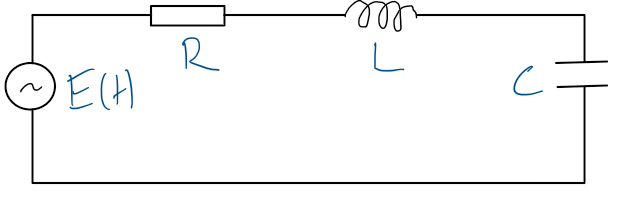
\includegraphics[width=0.5\textwidth]{SCHEMA13.png}
    \caption{Schema du pont diviseur de tension}
    \label{fig:SCHEMA13}
\end{figure}

\begin{figure}[!htb]
    \centering
    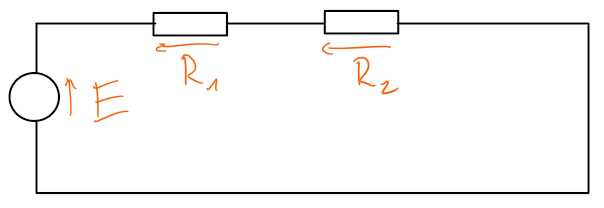
\includegraphics[width=0.5\textwidth]{SCHEMA14.png}
    \caption{Schema du montage}
    \label{fig:SCHEMA14}
\end{figure}

On a un pont diviseur de tension : 
\begin{eqnarray*}
    u_{cm} = \frac{Z_{c}}{Z_{R} + Z_{L} + Z_{c}}E \\
    = \frac{\frac{1}{jc \omega }}{R + j (L \omega -\frac{1}{c \omega })} E \\
    = \frac{E}{1 + jRc \omega  -LC \omega^{2}} \\
    \implies U_{cm} = \lvert u_{cm} \rvert = \frac{E}{\sqrt{(1-LC \omega)^{2} + (RC \omega )^{2}}} \\
    U_{m}( \omega0) = E \\
    U_{m} ( \omega \to \inf ) = 0 \\
    \text{ On pose } \omega_{0} \frac{1}{\sqrt{LC}} ; Q = \frac{L \omega_{0}}{R} \text{ et } x = \frac{\omega }{\omega _{0}} \\
    u_{cm} = \frac{E}{\sqrt{(1- \frac{\omega }{\omega _{0}}^{2})^{2}} + \frac{\omega }{Q \omega _{0}}^{2}} \\
    \implies u_{cm} = \frac{E}{\sqrt{(1-x^{2})^{2}}+ \frac{x}{Q}^{2}} \\
    \implies u_{cm} = \frac{E}{D} \\
    \implies \frac{d}{dx}D^{2} = -4x (1-x^{2}) + \frac{2x}{Q^{2}}\\
    \implies \frac{d}{dx}D^{2} = 0 \implies 1-x^{2} = \frac{1}{2Q^{2}} \implies \omega_{r} = \omega_{0} \sqrt{1-\frac{1}{2Q^{2}}}
\end{eqnarray*}
On peut avoir résonance que si : 
\begin{eqnarray*}
    1-\frac{1}{2Q^{2}} >0 \\
    \implies 2Q^{2} >1 \\
    \implies Q > \frac{1}{\sqrt{2}}
\end{eqnarray*}

\begin{remark}[Existance de la résonance]
    ATTENTION : La résonance en intensité existe toujours mais la résonance en tension n'existe que pour \(Q > \frac{1}{\sqrt{2}}\).  
\end{remark}

